\section{基本文字测试}
\label{sec:1}
我叫肖晗宇,来自浙江大学计算机学院,热爱开源软件、旅行、摄影,推崇互助共享的精神理念。

My name is Xiao Hanyu, a student from Computer Science and Technology of Zhejiang University, I love open source software, travelling all over the world, photography, and so on. 

我喜欢\LaTeXe,也推荐大家来学习使用\LaTeXe,以下是比较不错的学习资源:

\begin{enumerate}
\item LaTeX companion
\item The TeXbook
\end{enumerate}


\section{图形图像测试}
\subsection{插图测试}
Hand in Hand:\ref{fig:hand_in_hand}
\begin{figure}[htbp]
\centerline{\includegraphics[width=0.6\textwidth]{images/hand_in_hand.png}}
\caption[]{\label{fig:hand_in_hand} 手拉手}
\end{figure}

\subsection{pgf/tikz绘图测试}
图\ref{fig:monotonic_chain}是用pgf/tikz宏包作的图形,用以说明计算几何相关定理。

\begin{figure}
\centering
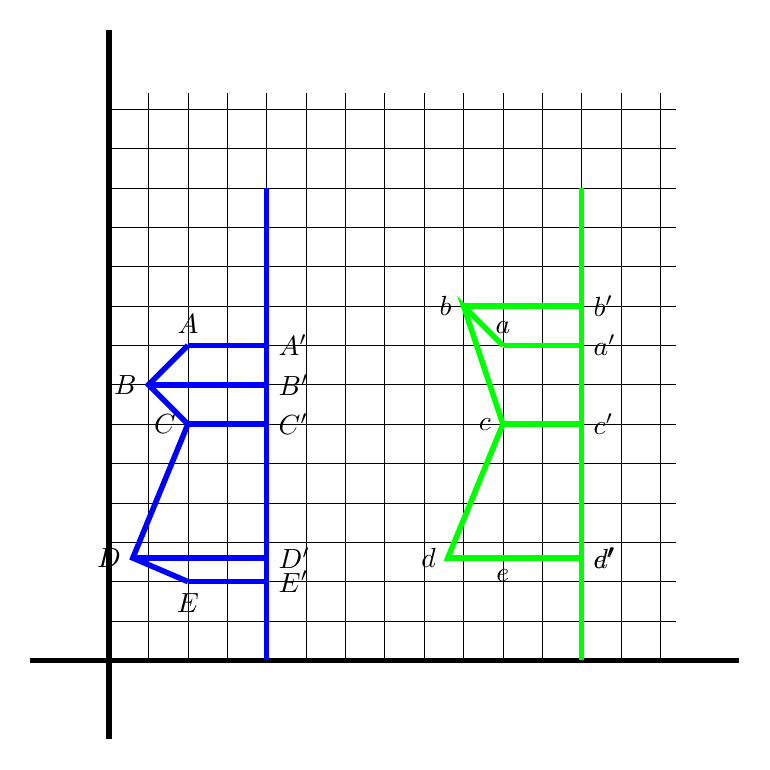
\begin{tikzpicture}[line width=2pt]
\draw (-1,0) -- (8,0);
\draw (0,-1) -- (0,8);
\draw[step=.5cm, very thin] (0,0) grid (7.2,7.2);

\coordinate [label=above:$A$] (A) at (1, 4);
\coordinate [label=left:$B$] (B) at (0.5, 3.5);
\coordinate [label=left:$C$] (C) at (1, 3);
\coordinate [label=left:$D$] (D) at (0.3, 1.3);
\coordinate [label=below:$E$] (E) at (1, 1);

\draw[blue] (A) -- (B) -- (C)  -- (D) -- (E);
\draw[blue] (2, 0) -- (2, 6);

\coordinate [label=right:$A'$] (A') at (2, 4);
\coordinate [label=right:$B'$] (B') at (2, 3.5);
\coordinate [label=right:$C'$] (C') at (2, 3);
\coordinate [label=right:$D'$] (D') at (2, 1.3);
\coordinate [label=right:$E'$] (E') at (2, 1);

\draw[blue] (A) -- (A');
\draw[blue] (B) -- (B');
\draw[blue] (C) -- (C');
\draw[blue] (D) -- (D');
\draw[blue] (E) -- (E');

\coordinate [label=above:$a$] (a) at (5, 4);
\coordinate [label=left:$b$] (b) at (4.5, 4.5);
\coordinate [label=left:$c$] (c) at (5, 3);
\coordinate [label=left:$d$] (d) at (4.3, 1.3);
\coordinate [label=below:$e$] (e) at (5, 1.3);

\draw[green] (a) -- (b) -- (c)  -- (d) -- (e);
\draw[green] (6, 0) -- (6, 6);

\coordinate [label=right:$a'$] (a') at (6, 4);
\coordinate [label=right:$b'$] (b') at (6, 4.5);
\coordinate [label=right:$c'$] (c') at (6, 3);
\coordinate [label=right:$d'$] (d') at (6, 1.3);
\coordinate [label=right:$e'$] (e') at (6, 1.3);

\draw[green] (a) -- (a');
\draw[green] (b) -- (b');
\draw[green] (c) -- (c');
\draw[green] (d) -- (d');
\draw[green] (e) -- (e');
\end{tikzpicture}
\caption{Monotonic polygonal chains}
\label{fig:monotonic_chain}
\end{figure}

\section{表格测试}
\begin{table}[htbp]
  \centering
  \begin{tabular}[htbp]{r|l}
    \toprule
    日期 & 任务 \\
    \midrule
    2011.5 & 完善此份文档 \\
    2011.6 & 完善安装脚本 \\
    \bottomrule
  \end{tabular}
  \caption{表格}
  \label{tab:table1}
\end{table}

\section{源代码高亮测试}

以下是\href{http://acm.zju.edu.cn/onlinejudge/showProblem.do?problemCode=1372}{ZOJ 1372}的解题c++代码:

\begin{lstlisting}[language=c++]
#include <iostream>
#include <string>
using namespace std;
 
const long max_points = 100;
const long infinity = 1000001;
 
int p, r, length, g[max_points][max_points];
bool flag;
 
class vertex
{
public:
    int distance;
    bool visited;
};
 
vertex v[max_points];
 
void initial()
{
    for(int i = 1; i <= p; i++)
        for(int j = 1; j <= p; j++)
            g[i][j] = infinity;
}
 
void prim(int origin)
{
    int temp_min;
    int temp_v = 0;
    int sum = 0;
 
    for(int i = 1; i <= p; i++)
    {
        v[i].distance = g[i][origin];
        v[i].visited = false;
    }
 
    v[origin].distance = 0;
    v[origin].visited = true;
 
    sum++;
 
    while (sum < p)
    {
        temp_min = infinity;
        for(int i = 1; i <= p; i++)
            if(v[i].visited == false && v[i].distance < temp_min)
            {
                temp_min = v[i].distance;
                temp_v = i;
            }
         
        if(temp_min < infinity)
        {
            length += v[temp_v].distance;
            v[temp_v].visited = true;
            sum++;
        }
        else
        {
            flag = true;
            break;
        }
 
        for(int i = 1; i <= p; i++)
        {
            if(v[i].visited == false && v[i].distance > g[i][temp_v])
            {
                v[i].distance = g[i][temp_v];
            }
        }
    }
}
 
int main(int argc, char *argv[])
{
    int a, b, c;
 
    while(cin >> p)
    {
        if(p == 0)
            break;
        cin >> r;
 
        initial();
 
        for(int i = 0; i < r; i++)
        {
            cin >> a >> b >> c;
            if(c < g[a][b])
                g[a][b] = g[b][a] = c;
        }
        length = 0;
        prim(1);
 
        cout << length << endl;
    }
 
    return 0;
} 
\end{lstlisting}

\section{数学公式测试}

著名的爱因斯坦质能方程(\ref{eq:emc2}):

\begin{equation}
  \label{eq:emc2}
  E=mc^2
\end{equation}

计算$f(x)=x^2$的不定积分(\ref{eq:2}):

\begin{equation}
  \label{eq:2}
  \int x^2 dx = \frac{1}{3} x^3
\end{equation}
\section{参考文件测试}
参考文件最好使用bibtex,关于bibtex的使用方法,你可以自行查阅相关文献。

这里是参考文献\cite{c_minigui}
